Automatizaci\'on de Procesos Rob\'oticos (Robotic Process Automation, RPA) \cite{Bataller2017} es una metodolog\'ia que tiene por objetivo la automatizaci\'on de procesos repetitivos usando robots de software, haciendo uso de procesamiento de im\'agenes, se identifican los elementos de la interfaz gr\'afica con los que interact\'ua el usuario, y un monitor de los dispositivos de entrada y salida para identificar la acci\'on realizada por \'el\cite{Bataller2017}. Sin embargo, al haber un cambio en la interfaz gr\'afica de usuario, del software utilizado, el RPA no lo puede procesar, por lo que tampoco puede realizar la tarea programada, considerando este problema, una posible soluci\'on es la mezcla de RPA con t\'ecnicas de inteligencia artificial y aprendizaje m\'aquina, permitiendo una mejora y adaptaci\'on a los cambios en el proceso ya establecido\cite{vanderAalst2018, Mohanty2018}.


El principal uso para el RPA son los procesos empresariales de fianzas y
 contabilidad, banca, mercados capitales y seguros\cite{Mohanty2018} ya que 
 se realizan en computadoras, sin embargo, no se ve limitado a esto, ya que 
 tambi\'en se est\'an explorando otras aplicaciones, por ejemplo, 
 supervisi\'on de campos de agricultura con drones\cite{inbook}.
 

El software UIPath Studio es un software que ofrece una interfaz gr\'afica para automatizar las tareas con RPA facilitando la implementaci\'on de este\cite{Dines2018}. En \cite{8479511} muestran una comparativa entre UIPath Studio, Automation Anywhere y Blue Prism, desarrollos de software que permiten la implementaci\'on de RPA, con la intenci\'on de que el lector pueda elegir la mejor herramienta dependiendo de sus necesidades. En la figura \ref{fig:uipath} se muestra la interfaz gr\'afica de UIPath.

 
\begin{figure}[h]
\centering
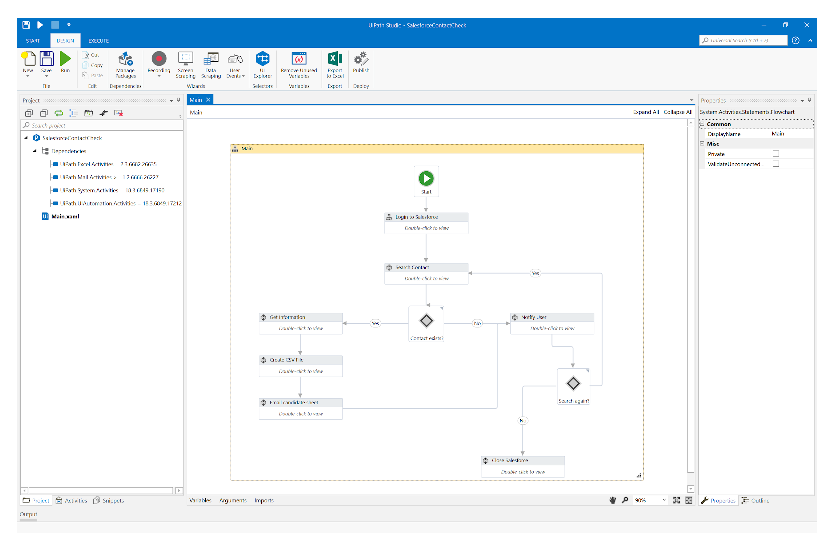
\includegraphics[width=0.8\columnwidth]{chap2/Imagenes/rpauipath.eps}
\caption{Interfaz de usuario de UIPath\cite{Dines2018}.}
\label{fig:uipath}
\end{figure}